\subsection{Конфигурация на на микроконтролера}

\subsubsection{Стартиране }

Написан е прост стартиращ скрипт на ARM assembly за целите на проекта ни, който инициализира SP на процесора и инициализира PC= Resethandler.
Скрипта дефинира символите от таблицата за прекъсванията, като .weak референции, към DefaultHandler, който изпълнява безкраен празен цикъл.
Този скрипт има за цел да инициализира .bss секцията на контролера,
както и всички статични променливи, като използва позициите генерирани от линкерният скрипт.
И да извика функцията за Системна инициализация, след което се извиква main финкцията.

\subsubsection{Системна инициализация}

В тази фаза се налага да инициализираме системният часовник.
В нашият случай ще инициализираме системният часовник. 
Тъй като при стартиране се използва високочестотният вътрешен осцилатор (HSI), който е
неточен и може да доведе до синхроннизационни проблеми при асинхронни комуникации 
с висок baud-rate каот UART.
Поради тази причина се налага инициализирането на системният часовник използваки 
високочестотният външен осцилатор (HSE) като времева основа, тъй-като е много по прецизен.
високочестотният външен осцилатор (HSE) на платката е с честота 8MHz, затова използваме
хардуерният PLL модул, за увеличаване на честотата, като използваме следните настройки 
\begin{verbatim}
    (PLL_M=8, PLL_N=336, PLL_P=2, PLL_Q=7)
\end{verbatim}
, като така получаваме честотата на системният часовник 168MHz.
След което инициализираме делителите на честота за отделните шини:
\begin{verbatim}
    (AHB_Prescaler=1, APB1_Prescaler=4, APB2_Prescaler=2).
\end{verbatim}
След настройката на часовниците получаваме следните честоти за отделните шини (\autoref{fig:frequencies})

\begin{figure}[htpb!]
    \centering
    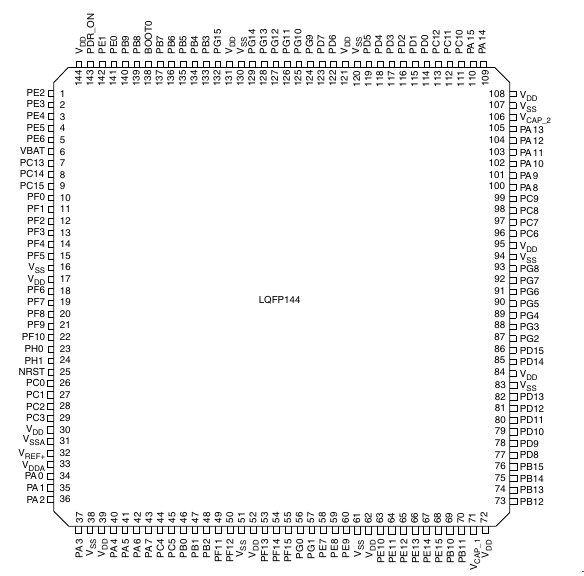
\includegraphics[width=0.5\textwidth]{mcu_pinout}
    \caption{Наименования на изведените пинове през използваният пакет}
    \label{fig:frequencies}
\end{figure}
 

